% Options for packages loaded elsewhere
% Options for packages loaded elsewhere
\PassOptionsToPackage{unicode}{hyperref}
\PassOptionsToPackage{hyphens}{url}
\PassOptionsToPackage{dvipsnames,svgnames,x11names}{xcolor}
%
\documentclass[
  spanish,
  11pt,
  a4paper,
  DIV=11,
  numbers=noendperiod]{scrartcl}
\usepackage{xcolor}
\usepackage[margin=2.5cm]{geometry}
\usepackage{amsmath,amssymb}
\setcounter{secnumdepth}{5}
\usepackage{iftex}
\ifPDFTeX
  \usepackage[T1]{fontenc}
  \usepackage[utf8]{inputenc}
  \usepackage{textcomp} % provide euro and other symbols
\else % if luatex or xetex
  \usepackage{unicode-math} % this also loads fontspec
  \defaultfontfeatures{Scale=MatchLowercase}
  \defaultfontfeatures[\rmfamily]{Ligatures=TeX,Scale=1}
\fi
\usepackage{lmodern}
\ifPDFTeX\else
  % xetex/luatex font selection
  \setmainfont[]{Times New Roman}
\fi
% Use upquote if available, for straight quotes in verbatim environments
\IfFileExists{upquote.sty}{\usepackage{upquote}}{}
\IfFileExists{microtype.sty}{% use microtype if available
  \usepackage[]{microtype}
  \UseMicrotypeSet[protrusion]{basicmath} % disable protrusion for tt fonts
}{}
\makeatletter
\@ifundefined{KOMAClassName}{% if non-KOMA class
  \IfFileExists{parskip.sty}{%
    \usepackage{parskip}
  }{% else
    \setlength{\parindent}{0pt}
    \setlength{\parskip}{6pt plus 2pt minus 1pt}}
}{% if KOMA class
  \KOMAoptions{parskip=half}}
\makeatother
% Make \paragraph and \subparagraph free-standing
\makeatletter
\ifx\paragraph\undefined\else
  \let\oldparagraph\paragraph
  \renewcommand{\paragraph}{
    \@ifstar
      \xxxParagraphStar
      \xxxParagraphNoStar
  }
  \newcommand{\xxxParagraphStar}[1]{\oldparagraph*{#1}\mbox{}}
  \newcommand{\xxxParagraphNoStar}[1]{\oldparagraph{#1}\mbox{}}
\fi
\ifx\subparagraph\undefined\else
  \let\oldsubparagraph\subparagraph
  \renewcommand{\subparagraph}{
    \@ifstar
      \xxxSubParagraphStar
      \xxxSubParagraphNoStar
  }
  \newcommand{\xxxSubParagraphStar}[1]{\oldsubparagraph*{#1}\mbox{}}
  \newcommand{\xxxSubParagraphNoStar}[1]{\oldsubparagraph{#1}\mbox{}}
\fi
\makeatother

\usepackage{color}
\usepackage{fancyvrb}
\newcommand{\VerbBar}{|}
\newcommand{\VERB}{\Verb[commandchars=\\\{\}]}
\DefineVerbatimEnvironment{Highlighting}{Verbatim}{commandchars=\\\{\}}
% Add ',fontsize=\small' for more characters per line
\usepackage{framed}
\definecolor{shadecolor}{RGB}{241,243,245}
\newenvironment{Shaded}{\begin{snugshade}}{\end{snugshade}}
\newcommand{\AlertTok}[1]{\textcolor[rgb]{0.68,0.00,0.00}{#1}}
\newcommand{\AnnotationTok}[1]{\textcolor[rgb]{0.37,0.37,0.37}{#1}}
\newcommand{\AttributeTok}[1]{\textcolor[rgb]{0.40,0.45,0.13}{#1}}
\newcommand{\BaseNTok}[1]{\textcolor[rgb]{0.68,0.00,0.00}{#1}}
\newcommand{\BuiltInTok}[1]{\textcolor[rgb]{0.00,0.23,0.31}{#1}}
\newcommand{\CharTok}[1]{\textcolor[rgb]{0.13,0.47,0.30}{#1}}
\newcommand{\CommentTok}[1]{\textcolor[rgb]{0.37,0.37,0.37}{#1}}
\newcommand{\CommentVarTok}[1]{\textcolor[rgb]{0.37,0.37,0.37}{\textit{#1}}}
\newcommand{\ConstantTok}[1]{\textcolor[rgb]{0.56,0.35,0.01}{#1}}
\newcommand{\ControlFlowTok}[1]{\textcolor[rgb]{0.00,0.23,0.31}{\textbf{#1}}}
\newcommand{\DataTypeTok}[1]{\textcolor[rgb]{0.68,0.00,0.00}{#1}}
\newcommand{\DecValTok}[1]{\textcolor[rgb]{0.68,0.00,0.00}{#1}}
\newcommand{\DocumentationTok}[1]{\textcolor[rgb]{0.37,0.37,0.37}{\textit{#1}}}
\newcommand{\ErrorTok}[1]{\textcolor[rgb]{0.68,0.00,0.00}{#1}}
\newcommand{\ExtensionTok}[1]{\textcolor[rgb]{0.00,0.23,0.31}{#1}}
\newcommand{\FloatTok}[1]{\textcolor[rgb]{0.68,0.00,0.00}{#1}}
\newcommand{\FunctionTok}[1]{\textcolor[rgb]{0.28,0.35,0.67}{#1}}
\newcommand{\ImportTok}[1]{\textcolor[rgb]{0.00,0.46,0.62}{#1}}
\newcommand{\InformationTok}[1]{\textcolor[rgb]{0.37,0.37,0.37}{#1}}
\newcommand{\KeywordTok}[1]{\textcolor[rgb]{0.00,0.23,0.31}{\textbf{#1}}}
\newcommand{\NormalTok}[1]{\textcolor[rgb]{0.00,0.23,0.31}{#1}}
\newcommand{\OperatorTok}[1]{\textcolor[rgb]{0.37,0.37,0.37}{#1}}
\newcommand{\OtherTok}[1]{\textcolor[rgb]{0.00,0.23,0.31}{#1}}
\newcommand{\PreprocessorTok}[1]{\textcolor[rgb]{0.68,0.00,0.00}{#1}}
\newcommand{\RegionMarkerTok}[1]{\textcolor[rgb]{0.00,0.23,0.31}{#1}}
\newcommand{\SpecialCharTok}[1]{\textcolor[rgb]{0.37,0.37,0.37}{#1}}
\newcommand{\SpecialStringTok}[1]{\textcolor[rgb]{0.13,0.47,0.30}{#1}}
\newcommand{\StringTok}[1]{\textcolor[rgb]{0.13,0.47,0.30}{#1}}
\newcommand{\VariableTok}[1]{\textcolor[rgb]{0.07,0.07,0.07}{#1}}
\newcommand{\VerbatimStringTok}[1]{\textcolor[rgb]{0.13,0.47,0.30}{#1}}
\newcommand{\WarningTok}[1]{\textcolor[rgb]{0.37,0.37,0.37}{\textit{#1}}}

\usepackage{longtable,booktabs,array}
\usepackage{calc} % for calculating minipage widths
% Correct order of tables after \paragraph or \subparagraph
\usepackage{etoolbox}
\makeatletter
\patchcmd\longtable{\par}{\if@noskipsec\mbox{}\fi\par}{}{}
\makeatother
% Allow footnotes in longtable head/foot
\IfFileExists{footnotehyper.sty}{\usepackage{footnotehyper}}{\usepackage{footnote}}
\makesavenoteenv{longtable}
\usepackage{graphicx}
\makeatletter
\newsavebox\pandoc@box
\newcommand*\pandocbounded[1]{% scales image to fit in text height/width
  \sbox\pandoc@box{#1}%
  \Gscale@div\@tempa{\textheight}{\dimexpr\ht\pandoc@box+\dp\pandoc@box\relax}%
  \Gscale@div\@tempb{\linewidth}{\wd\pandoc@box}%
  \ifdim\@tempb\p@<\@tempa\p@\let\@tempa\@tempb\fi% select the smaller of both
  \ifdim\@tempa\p@<\p@\scalebox{\@tempa}{\usebox\pandoc@box}%
  \else\usebox{\pandoc@box}%
  \fi%
}
% Set default figure placement to htbp
\def\fps@figure{htbp}
\makeatother



\ifLuaTeX
\usepackage[bidi=basic]{babel}
\else
\usepackage[bidi=default]{babel}
\fi
\ifPDFTeX
\else
\babelfont{rm}[]{Times New Roman}
\fi
% get rid of language-specific shorthands (see #6817):
\let\LanguageShortHands\languageshorthands
\def\languageshorthands#1{}


\setlength{\emergencystretch}{3em} % prevent overfull lines

\providecommand{\tightlist}{%
  \setlength{\itemsep}{0pt}\setlength{\parskip}{0pt}}



 


\usepackage{booktabs}
\usepackage{longtable}
\usepackage{array}
\usepackage{multirow}
\usepackage{wrapfig}
\usepackage{float}
\usepackage{colortbl}
\usepackage{pdflscape}
\usepackage{tabu}
\usepackage{threeparttable}
\usepackage{threeparttablex}
\usepackage[normalem]{ulem}
\usepackage{makecell}
\usepackage{xcolor}
\usepackage[hidelinks]{hyperref}
\KOMAoption{captions}{tableheading}
\makeatletter
\@ifpackageloaded{caption}{}{\usepackage{caption}}
\AtBeginDocument{%
\ifdefined\contentsname
  \renewcommand*\contentsname{Tabla de contenidos}
\else
  \newcommand\contentsname{Tabla de contenidos}
\fi
\ifdefined\listfigurename
  \renewcommand*\listfigurename{Listado de Figuras}
\else
  \newcommand\listfigurename{Listado de Figuras}
\fi
\ifdefined\listtablename
  \renewcommand*\listtablename{Listado de Tablas}
\else
  \newcommand\listtablename{Listado de Tablas}
\fi
\ifdefined\figurename
  \renewcommand*\figurename{Figura}
\else
  \newcommand\figurename{Figura}
\fi
\ifdefined\tablename
  \renewcommand*\tablename{Tabla}
\else
  \newcommand\tablename{Tabla}
\fi
}
\@ifpackageloaded{float}{}{\usepackage{float}}
\floatstyle{ruled}
\@ifundefined{c@chapter}{\newfloat{codelisting}{h}{lop}}{\newfloat{codelisting}{h}{lop}[chapter]}
\floatname{codelisting}{Listado}
\newcommand*\listoflistings{\listof{codelisting}{Listado de Listados}}
\makeatother
\makeatletter
\makeatother
\makeatletter
\@ifpackageloaded{caption}{}{\usepackage{caption}}
\@ifpackageloaded{subcaption}{}{\usepackage{subcaption}}
\makeatother
\usepackage{bookmark}
\IfFileExists{xurl.sty}{\usepackage{xurl}}{} % add URL line breaks if available
\urlstyle{same}
\hypersetup{
  pdftitle={Cluster-Discriminante},
  pdfauthor={Santos G},
  pdflang={es},
  colorlinks=true,
  linkcolor={blue},
  filecolor={Maroon},
  citecolor={Blue},
  urlcolor={Blue},
  pdfcreator={LaTeX via pandoc}}


\title{Cluster-Discriminante}
\author{Santos G}
\date{}
\begin{document}
\maketitle

\renewcommand*\contentsname{Tabla de contenidos}
{
\hypersetup{linkcolor=}
\setcounter{tocdepth}{2}
\tableofcontents
}

\section{Contexto del proyecto}\label{contexto-del-proyecto}

La finalidad de esta guía es mostrar un flujo reproducible y profesional
para realizar análisis de agrupamiento (clustering) sobre variables
continuas en un contexto ambiental/biológico. Aprenderás a preparar los
datos, establecer la tendencia a agruparse, seleccionar el número óptimo
de clústeres, ejecutar clustering jerárquico y particional (k-means),
evaluar la calidad del agrupamiento y describir los grupos desde el
punto de vista estadístico y práctico.

\section{Carga de librerías y
dataset}\label{carga-de-libreruxedas-y-dataset}

\begin{Shaded}
\begin{Highlighting}[numbers=left,,]
\CommentTok{\# Librerías necesarias}
\FunctionTok{library}\NormalTok{(tidyverse)    }\CommentTok{\# manipulación de datos y ggplot2}
\FunctionTok{library}\NormalTok{(cluster)      }\CommentTok{\# silhouette, pam, etc.}
\FunctionTok{library}\NormalTok{(factoextra)   }\CommentTok{\# funciones para visualizar clustering y gap statistic}
\FunctionTok{library}\NormalTok{(NbClust)      }\CommentTok{\# selección de k por múltiples índices}
\FunctionTok{library}\NormalTok{(clusterCrit)  }\CommentTok{\# índices de validación (opcional)}
\FunctionTok{library}\NormalTok{(dendextend)   }\CommentTok{\# manipular dendrogramas}
\FunctionTok{library}\NormalTok{(knitr)        }\CommentTok{\# kable()}
\FunctionTok{library}\NormalTok{(kableExtra)   }\CommentTok{\# estilo de tablas}
\FunctionTok{library}\NormalTok{(clustertend)  }\CommentTok{\# get\_clust\_tendency (Hopkins)}

\CommentTok{\# Cargar dataset y preparar}
\FunctionTok{data}\NormalTok{(}\StringTok{"USArrests"}\NormalTok{)}
\NormalTok{A\_raw }\OtherTok{\textless{}{-}}\NormalTok{ USArrests }\SpecialCharTok{\%\textgreater{}\%} \FunctionTok{as\_tibble}\NormalTok{(}\AttributeTok{rownames =} \StringTok{"region"}\NormalTok{)}

\CommentTok{\# Guardar copia original para auditoría}
\NormalTok{A\_orig }\OtherTok{\textless{}{-}}\NormalTok{ A\_raw}

\CommentTok{\# Selección de variables numéricas y escalado (estandarizar)}
\NormalTok{num\_vars }\OtherTok{\textless{}{-}}\NormalTok{ A\_raw }\SpecialCharTok{\%\textgreater{}\%} \FunctionTok{select}\NormalTok{(Murder, Assault, UrbanPop, Rape)}
\NormalTok{num\_scaled }\OtherTok{\textless{}{-}} \FunctionTok{scale}\NormalTok{(num\_vars) }\SpecialCharTok{\%\textgreater{}\%} \FunctionTok{as\_tibble}\NormalTok{() }\SpecialCharTok{\%\textgreater{}\%} \FunctionTok{setNames}\NormalTok{(}\FunctionTok{colnames}\NormalTok{(num\_vars))}
\end{Highlighting}
\end{Shaded}

\section{Preparación de la matriz para
clustering}\label{preparaciuxf3n-de-la-matriz-para-clustering}

\begin{Shaded}
\begin{Highlighting}[numbers=left,,]
\NormalTok{summary\_tbl }\OtherTok{\textless{}{-}}\NormalTok{ num\_vars }\SpecialCharTok{\%\textgreater{}\%}
\FunctionTok{summarise}\NormalTok{(}\FunctionTok{across}\NormalTok{(}\FunctionTok{everything}\NormalTok{(), }\FunctionTok{list}\NormalTok{(}\AttributeTok{mean =} \SpecialCharTok{\textasciitilde{}}\FunctionTok{mean}\NormalTok{(.), }\AttributeTok{sd =} \SpecialCharTok{\textasciitilde{}}\FunctionTok{sd}\NormalTok{(.),}
\AttributeTok{min =} \SpecialCharTok{\textasciitilde{}}\FunctionTok{min}\NormalTok{(.), }\AttributeTok{max =} \SpecialCharTok{\textasciitilde{}}\FunctionTok{max}\NormalTok{(.)))) }\SpecialCharTok{\%\textgreater{}\%}
\FunctionTok{pivot\_longer}\NormalTok{(}\FunctionTok{everything}\NormalTok{(), }\AttributeTok{names\_to =} \FunctionTok{c}\NormalTok{(}\StringTok{"variable"}\NormalTok{,}\StringTok{"stat"}\NormalTok{), }\AttributeTok{names\_sep =} \StringTok{"\_"}\NormalTok{) }\SpecialCharTok{\%\textgreater{}\%}
\FunctionTok{pivot\_wider}\NormalTok{(}\AttributeTok{names\_from =}\NormalTok{ stat, }\AttributeTok{values\_from =}\NormalTok{ value) }\SpecialCharTok{\%\textgreater{}\%}
\FunctionTok{select}\NormalTok{(variable, mean, sd, min, max)}

\NormalTok{knitr}\SpecialCharTok{::}\FunctionTok{kable}\NormalTok{(summary\_tbl, }\AttributeTok{digits =} \DecValTok{3}\NormalTok{)}
\end{Highlighting}
\end{Shaded}

\begin{longtable}[]{@{}lrrrr@{}}

\caption{\label{tbl-clust-prep}Resumen numérico de variables para
clustering}

\tabularnewline

\toprule\noalign{}
variable & mean & sd & min & max \\
\midrule\noalign{}
\endhead
\bottomrule\noalign{}
\endlastfoot
Murder & 7.788 & 4.356 & 0.8 & 17.4 \\
Assault & 170.760 & 83.338 & 45.0 & 337.0 \\
UrbanPop & 65.540 & 14.475 & 32.0 & 91.0 \\
Rape & 21.232 & 9.366 & 7.3 & 46.0 \\

\end{longtable}

El conjunto de variables seleccionadas para el análisis de agrupamiento
incluye indicadores sociales y de criminalidad: tasas de homicidios
(Murder), asaltos (Assault), porcentaje de población urbana (UrbanPop) y
delitos sexuales (Rape).

De acuerdo con el resumen estadístico (ver Tabla~\ref{tbl-clust-prep}),
se observa una variabilidad considerable entre estados:

\begin{itemize}
\item
  Murder presenta una media de 7.79 delitos con valores entre 0.8 y 17.4
  , lo que evidencia fuertes contrastes en las tasas de homicidios a
  nivel estatal.
\item
  Assault (asaltos) muestra la mayor dispersión (SD = 83.3 ), con un
  rango amplio entre 45 y 337 incidentes, indicando marcadas diferencias
  en la incidencia de violencia física.
\item
  UrbanPop, porcentaje de población urbana, promedia 65.5 \% (rango: 32
  -- 91 ), mostrando una distribución relativamente homogénea, aunque
  con algunos estados menos urbanizados.
\item
  Finalmente, Rape presenta un promedio de 21.2 casos por 100.000
  habitantes y una desviación estándar de 9.4 , lo que sugiere
  heterogeneidad en la prevalencia de este tipo de delitos.
\end{itemize}

En conjunto, la amplitud de los rangos y desviaciones indica una base de
datos con suficiente variabilidad para aplicar técnicas de agrupamiento
y explorar posibles perfiles regionales de criminalidad y urbanización.

\begin{Shaded}
\begin{Highlighting}[numbers=left,,]
\CommentTok{\# Hopkins}
\FunctionTok{set.seed}\NormalTok{(}\DecValTok{42}\NormalTok{)}
\NormalTok{hopkins\_stat }\OtherTok{\textless{}{-}} \FunctionTok{get\_clust\_tendency}\NormalTok{(num\_scaled, }\AttributeTok{n =} \FunctionTok{nrow}\NormalTok{(num\_scaled) }\SpecialCharTok{{-}} \DecValTok{1}\NormalTok{, }
                                   \AttributeTok{graph =}\ConstantTok{FALSE}\NormalTok{)}\SpecialCharTok{$}\NormalTok{hopkins\_stat}

\NormalTok{hopkins\_res }\OtherTok{\textless{}{-}} \FunctionTok{tibble}\NormalTok{(}\AttributeTok{test =} \StringTok{"Hopkins"}\NormalTok{, }\AttributeTok{value =} \FunctionTok{round}\NormalTok{(hopkins\_stat, }\DecValTok{3}\NormalTok{))}
\NormalTok{knitr}\SpecialCharTok{::}\FunctionTok{kable}\NormalTok{(hopkins\_res, }\AttributeTok{caption =} \StringTok{""}\NormalTok{)}
\end{Highlighting}
\end{Shaded}

\begin{longtable}[]{@{}lr@{}}

\caption{\label{tbl-clust-hopkins}Test de tendencia al agrupamiento
(Hopkins)}

\tabularnewline

\toprule\noalign{}
test & value \\
\midrule\noalign{}
\endhead
\bottomrule\noalign{}
\endlastfoot
Hopkins & 0.608 \\

\end{longtable}

El test de tendencia al agrupamiento de Hopkins (ver
Tabla~\ref{tbl-clust-hopkins}) arrojó un valor de 0.608 . Este
estadístico evalúa si los datos presentan una estructura de agrupamiento
no aleatoria. Donde, valores cercanos a 0 indican una fuerte tendencia a
agruparse, mientras que valores iguales o mayores oa 0.5 sugieren una
distribución aleatoria. En este caso, el valor obtenido ( 0.608 ) se
aproxima a 0.5, lo que sugiere una estructura de agrupamiento débil en
el conjunto de datos. Esto implica que los estados de EE.UU. no se
diferencian en grupos muy definidos según las variables de criminalidad
y urbanización, aunque podrían existir subgrupos moderadamente
diferenciados que justifiquen la aplicación de métodos de clustering
exploratorio.

\section{Elección del número de clusters
(validación)}\label{elecciuxf3n-del-nuxfamero-de-clusters-validaciuxf3n}

\begin{Shaded}
\begin{Highlighting}[numbers=left,,]
\CommentTok{\# Distancia Euclidiana y Ward.D2}
\NormalTok{dist\_mat }\OtherTok{\textless{}{-}} \FunctionTok{dist}\NormalTok{(num\_scaled, }\AttributeTok{method =} \StringTok{"euclidean"}\NormalTok{)}
\NormalTok{hc }\OtherTok{\textless{}{-}} \FunctionTok{hclust}\NormalTok{(dist\_mat, }\AttributeTok{method =} \StringTok{"ward.D2"}\NormalTok{)}

\CommentTok{\# Silhouette promedio para k = 2..6 (kmeans)}
\NormalTok{sil\_vals }\OtherTok{\textless{}{-}} \FunctionTok{tibble}\NormalTok{(}\AttributeTok{k =} \DecValTok{2}\SpecialCharTok{:}\DecValTok{6}\NormalTok{, }\AttributeTok{sil\_avg =} \ConstantTok{NA\_real\_}\NormalTok{)}
\ControlFlowTok{for}\NormalTok{ (k }\ControlFlowTok{in} \DecValTok{2}\SpecialCharTok{:}\DecValTok{6}\NormalTok{) \{}
\NormalTok{km }\OtherTok{\textless{}{-}} \FunctionTok{kmeans}\NormalTok{(num\_scaled, }\AttributeTok{centers =}\NormalTok{ k, }\AttributeTok{nstart =} \DecValTok{50}\NormalTok{)}
\NormalTok{sil }\OtherTok{\textless{}{-}} \FunctionTok{silhouette}\NormalTok{(km}\SpecialCharTok{$}\NormalTok{cluster, dist\_mat)}
\NormalTok{sil\_vals}\SpecialCharTok{$}\NormalTok{sil\_avg[sil\_vals}\SpecialCharTok{$}\NormalTok{k }\SpecialCharTok{==}\NormalTok{ k] }\OtherTok{\textless{}{-}} \FunctionTok{mean}\NormalTok{(sil[, }\DecValTok{3}\NormalTok{])}
\NormalTok{\}}
\NormalTok{knitr}\SpecialCharTok{::}\FunctionTok{kable}\NormalTok{(sil\_vals, }\AttributeTok{digits =} \DecValTok{3}\NormalTok{)}
\end{Highlighting}
\end{Shaded}

\begin{longtable}[]{@{}rr@{}}

\caption{\label{tbl-clust-k}Silhouette promedio por número de clusters
(k)}

\tabularnewline

\toprule\noalign{}
k & sil\_avg \\
\midrule\noalign{}
\endhead
\bottomrule\noalign{}
\endlastfoot
2 & 0.408 \\
3 & 0.309 \\
4 & 0.340 \\
5 & 0.303 \\
6 & 0.286 \\

\end{longtable}

De acuerdo con los resultados del índice de Silhouette (ver
Tabla~\ref{tbl-clust-k}), el valor más alto se obtuvo para k = 2, con un
promedio de 0.408, lo que indica que esta partición presenta la mejor
cohesión interna y separación entre grupos. A medida que aumenta el
número de clústeres, el valor de la silueta disminuye progresivamente
(por ejemplo, 0.309 para \emph{k = 3} y 0.34 para \emph{k = 4}),
reflejando una menor nitidez en la estructura del agrupamiento.

\begin{Shaded}
\begin{Highlighting}[numbers=left,,]
\CommentTok{\# Gap statistic}
\FunctionTok{set.seed}\NormalTok{(}\DecValTok{42}\NormalTok{)}
\NormalTok{gap }\OtherTok{\textless{}{-}} \FunctionTok{clusGap}\NormalTok{(num\_scaled, }\AttributeTok{FUN =}\NormalTok{ kmeans, }\AttributeTok{K.max =} \DecValTok{6}\NormalTok{, }\AttributeTok{B =} \DecValTok{50}\NormalTok{)}
\FunctionTok{fviz\_gap\_stat}\NormalTok{(gap)  }\CommentTok{\# figura}
\end{Highlighting}
\end{Shaded}

\begin{figure}[H]

\centering{

\pandocbounded{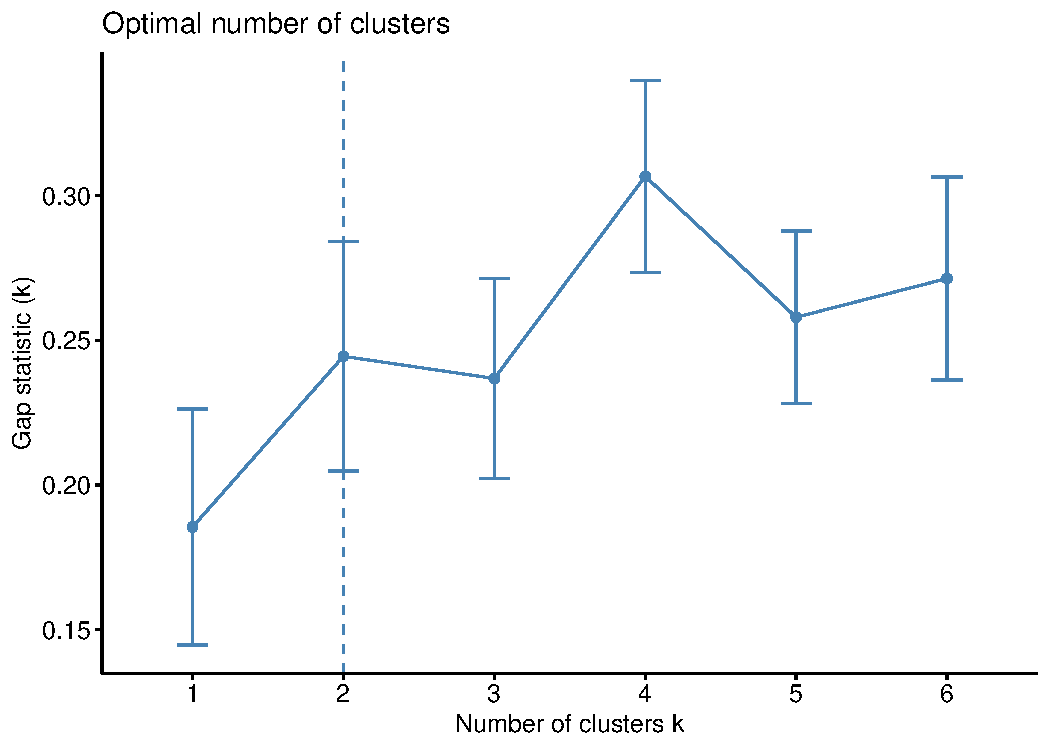
\includegraphics[keepaspectratio]{Cluster-Discriminante_files/figure-pdf/fig-clust-gap-1.pdf}}

}

\caption{\label{fig-clust-gap}Análisis del Gap statistic}

\end{figure}%

El análisis del \emph{Gap Statistic} (ver Figura~\ref{fig-clust-gap})
mostró un patrón coherente, con el valor máximo en torno a dos
clústeres, lo que respalda una estructura de dos grupos bien
diferenciados en el espacio morfológico.

\section{K-means}\label{k-means}

\begin{Shaded}
\begin{Highlighting}[numbers=left,,]
\CommentTok{\# Ejecutar k{-}means con el k elegido (aquí usamos el k con mayor sil\_avg)}
\NormalTok{k\_opt }\OtherTok{\textless{}{-}}\NormalTok{ sil\_vals}\SpecialCharTok{$}\NormalTok{k[}\FunctionTok{which.max}\NormalTok{(sil\_vals}\SpecialCharTok{$}\NormalTok{sil\_avg)]}
\FunctionTok{set.seed}\NormalTok{(}\DecValTok{42}\NormalTok{)}
\NormalTok{km\_res }\OtherTok{\textless{}{-}} \FunctionTok{kmeans}\NormalTok{(num\_scaled, }\AttributeTok{centers =}\NormalTok{ k\_opt, }\AttributeTok{nstart =} \DecValTok{50}\NormalTok{)}

\CommentTok{\# Añadir cluster al df original}
\NormalTok{df\_clust }\OtherTok{\textless{}{-}}\NormalTok{ A\_raw }\SpecialCharTok{\%\textgreater{}\%} \FunctionTok{mutate}\NormalTok{(}\AttributeTok{cluster\_k =} \FunctionTok{factor}\NormalTok{(km\_res}\SpecialCharTok{$}\NormalTok{cluster))}

\CommentTok{\# Visualizar clusters sobre PC1{-}PC2 (representación)}
\FunctionTok{fviz\_cluster}\NormalTok{(km\_res, }\AttributeTok{data =}\NormalTok{ num\_scaled, }\AttributeTok{geom =} \StringTok{"point"}\NormalTok{, }\AttributeTok{ellipse.type =} \StringTok{"norm"}\NormalTok{,}
\AttributeTok{palette =} \StringTok{"jco"}\NormalTok{, }\AttributeTok{ggtheme =} \FunctionTok{theme\_minimal}\NormalTok{())}
\end{Highlighting}
\end{Shaded}

\begin{figure}[H]

\centering{

\pandocbounded{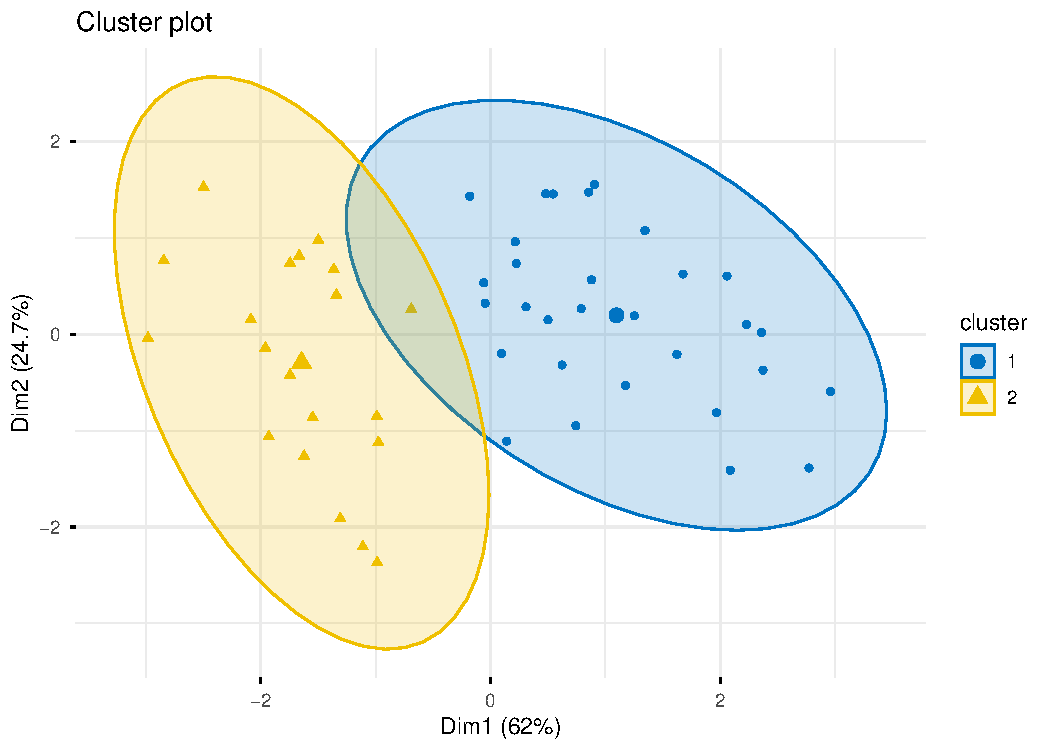
\includegraphics[keepaspectratio]{Cluster-Discriminante_files/figure-pdf/fig-clust-kmeans-1.pdf}}

}

\caption{\label{fig-clust-kmeans}K-means (k = 2) y representación en
PC1-PC2}

\end{figure}%

El gráfico de agrupamiento obtenido mediante el algoritmo k-means (ver
Figura~\ref{fig-clust-kmeans}) muestra la distribución de las
observaciones en el espacio definido por las dos primeras componentes
principales (Dim1 y Dim2), las cuales explican conjuntamente una
proporción considerable de la variabilidad total de los datos
(aproximadamente el 87\%).

Con k = 2 clústeres, se distinguen dos grupos principales bien
definidos, representados por las elipses de color azul (Cluster 1) y
amarillo (Cluster 2). El Cluster 1 agrupa observaciones con valores más
altos en la primera dimensión (Dim1), lo que sugiere un patrón
particular en las variables originales que contribuyen positivamente a
ese componente. Por su parte, el Cluster 2 se concentra hacia el extremo
opuesto de Dim1, reuniendo observaciones con valores más bajos en dicha
dimensión, lo cual indica diferencias sistemáticas respecto al grupo
azul.

La ligera superposición entre ambas elipses evidencia cierta similitud
parcial entre algunos estados de los dos grupos, aunque la separación
global es clara, lo que respalda la validez de la partición obtenida
mediante k-means.

\begin{Shaded}
\begin{Highlighting}[numbers=left,,]
\CommentTok{\# Calcular medias por grupo en variables escaladas}
\NormalTok{cluster\_summary }\OtherTok{\textless{}{-}}\NormalTok{ num\_scaled }\SpecialCharTok{\%\textgreater{}\%}
  \FunctionTok{mutate}\NormalTok{(}\AttributeTok{cluster =}\NormalTok{ km\_res}\SpecialCharTok{$}\NormalTok{cluster) }\SpecialCharTok{\%\textgreater{}\%}
  \FunctionTok{pivot\_longer}\NormalTok{(}\SpecialCharTok{{-}}\NormalTok{cluster, }\AttributeTok{names\_to =} \StringTok{"variable"}\NormalTok{, }\AttributeTok{values\_to =} \StringTok{"valor"}\NormalTok{) }\SpecialCharTok{\%\textgreater{}\%}
  \FunctionTok{group\_by}\NormalTok{(cluster, variable) }\SpecialCharTok{\%\textgreater{}\%}
  \FunctionTok{summarise}\NormalTok{(}\AttributeTok{mean =} \FunctionTok{mean}\NormalTok{(valor), }\AttributeTok{.groups =} \StringTok{"drop"}\NormalTok{) }\SpecialCharTok{\%\textgreater{}\%}
  \FunctionTok{pivot\_wider}\NormalTok{(}\AttributeTok{names\_from =}\NormalTok{ variable, }\AttributeTok{values\_from =}\NormalTok{ mean)}

\CommentTok{\# Reordenar etiquetas de clúster según la media de Murder}
\NormalTok{cluster\_order }\OtherTok{\textless{}{-}}\NormalTok{ cluster\_summary }\SpecialCharTok{\%\textgreater{}\%}
  \FunctionTok{mutate}\NormalTok{(}\AttributeTok{avg\_violence =}\NormalTok{ Murder) }\SpecialCharTok{\%\textgreater{}\%}
  \FunctionTok{arrange}\NormalTok{(avg\_violence) }\SpecialCharTok{\%\textgreater{}\%}
  \FunctionTok{mutate}\NormalTok{(}\AttributeTok{new\_cluster =} \FunctionTok{row\_number}\NormalTok{())}

\CommentTok{\# Crear un vector de equivalencia}
\NormalTok{mapping }\OtherTok{\textless{}{-}}\NormalTok{ cluster\_order}\SpecialCharTok{$}\NormalTok{new\_cluster}
\FunctionTok{names}\NormalTok{(mapping) }\OtherTok{\textless{}{-}}\NormalTok{ cluster\_order}\SpecialCharTok{$}\NormalTok{cluster}

\CommentTok{\# Reetiquetar clusters en los datos originales}
\NormalTok{df\_clust }\OtherTok{\textless{}{-}}\NormalTok{ A\_raw }\SpecialCharTok{\%\textgreater{}\%}
  \FunctionTok{mutate}\NormalTok{(}\AttributeTok{cluster\_k =} \FunctionTok{factor}\NormalTok{(mapping[km\_res}\SpecialCharTok{$}\NormalTok{cluster]))}

\CommentTok{\# Actualizar cluster\_summary con nuevas etiquetas}
\NormalTok{cluster\_summary }\OtherTok{\textless{}{-}}\NormalTok{ cluster\_summary }\SpecialCharTok{\%\textgreater{}\%}
  \FunctionTok{mutate}\NormalTok{(}\AttributeTok{cluster =}\NormalTok{ mapping[cluster]) }\SpecialCharTok{\%\textgreater{}\%}
  \FunctionTok{arrange}\NormalTok{(cluster)}

\CommentTok{\# Tabla con medias reordenadas}
\NormalTok{knitr}\SpecialCharTok{::}\FunctionTok{kable}\NormalTok{(cluster\_summary, }\AttributeTok{digits =} \DecValTok{2}\NormalTok{)}
\end{Highlighting}
\end{Shaded}

\begin{longtable}[]{@{}rrrrr@{}}

\caption{\label{tbl-clust-summary}Resumen comparativo de variables por
clúster}

\tabularnewline

\toprule\noalign{}
cluster & Assault & Murder & Rape & UrbanPop \\
\midrule\noalign{}
\endhead
\bottomrule\noalign{}
\endlastfoot
1 & -0.68 & -0.67 & -0.56 & -0.13 \\
2 & 1.01 & 1.00 & 0.85 & 0.20 \\

\end{longtable}

La Tabla~\ref{tbl-clust-summary} presenta las medias estandarizadas de
cada variable en los grupos identificados mediante k-means (k = 2 ).

El Cluster 1 muestra valores negativos en todas las variables (por
ejemplo, \emph{Assault} = -0.68 , \emph{Murder} = -0.67 , \emph{Rape} =
-0.56 ), lo que indica estados con niveles de criminalidad inferiores al
promedio nacional. Su valor en \emph{UrbanPop} ( -0.13 ) también se
sitúa ligeramente por debajo de la media, lo que sugiere una menor
proporción de población urbana.

En contraste, el Cluster 2 presenta valores positivos en todas las
variables (por ejemplo, \emph{Assault} = 1.01 , \emph{Murder} = 1 ,
\emph{Rape} = 0.85 ), indicando estados con mayores tasas de
criminalidad. Su leve incremento en \emph{UrbanPop} ( 0.2 ) apunta a una
tendencia hacia contextos más urbanizados, aunque esta diferencia es
menos marcada.

En conjunto, los resultados evidencian que la separación entre grupos
responde principalmente a un eje de intensidad delictiva, más que a
diferencias en urbanización o tamaño poblacional.

\section{Clustering jerárquico (HC)}\label{clustering-jeruxe1rquico-hc}

\begin{Shaded}
\begin{Highlighting}[numbers=left,,]
\CommentTok{\# Cortar el dendrograma en 2 grupos}
\NormalTok{grupos\_hc }\OtherTok{\textless{}{-}} \FunctionTok{cutree}\NormalTok{(hc, }\AttributeTok{k =} \DecValTok{2}\NormalTok{)}

\CommentTok{\# Calcular medias estandarizadas por grupo}
\NormalTok{hc\_summary }\OtherTok{\textless{}{-}}\NormalTok{ num\_scaled }\SpecialCharTok{\%\textgreater{}\%}
  \FunctionTok{mutate}\NormalTok{(}\AttributeTok{cluster =}\NormalTok{ grupos\_hc) }\SpecialCharTok{\%\textgreater{}\%}
  \FunctionTok{pivot\_longer}\NormalTok{(}\SpecialCharTok{{-}}\NormalTok{cluster, }\AttributeTok{names\_to =} \StringTok{"variable"}\NormalTok{, }\AttributeTok{values\_to =} \StringTok{"valor"}\NormalTok{) }\SpecialCharTok{\%\textgreater{}\%}
  \FunctionTok{group\_by}\NormalTok{(cluster, variable) }\SpecialCharTok{\%\textgreater{}\%}
  \FunctionTok{summarise}\NormalTok{(}\AttributeTok{mean =} \FunctionTok{mean}\NormalTok{(valor), }\AttributeTok{.groups =} \StringTok{"drop"}\NormalTok{) }\SpecialCharTok{\%\textgreater{}\%}
  \FunctionTok{pivot\_wider}\NormalTok{(}\AttributeTok{names\_from =}\NormalTok{ variable, }\AttributeTok{values\_from =}\NormalTok{ mean)}

\CommentTok{\# Mostrar tabla resumen}
\NormalTok{knitr}\SpecialCharTok{::}\FunctionTok{kable}\NormalTok{(hc\_summary, }\AttributeTok{digits =} \DecValTok{2}\NormalTok{)}
\end{Highlighting}
\end{Shaded}

\begin{longtable}[]{@{}rrrrr@{}}

\caption{\label{tbl-hc-summary}Resumen comparativo de variables por
clúster (clustering jerárquico)}

\tabularnewline

\toprule\noalign{}
cluster & Assault & Murder & Rape & UrbanPop \\
\midrule\noalign{}
\endhead
\bottomrule\noalign{}
\endlastfoot
1 & 1.06 & 1.04 & 0.85 & 0.19 \\
2 & -0.65 & -0.64 & -0.52 & -0.12 \\

\end{longtable}

La Tabla~\ref{tbl-hc-summary} resume las medias estandarizadas de las
variables consideradas en el análisis jerárquico.

El Cluster 1 presenta valores positivos en todas las variables
(\emph{Assault} = 1.06 , \emph{Murder} = 1.04 , \emph{Rape} = 0.85 ,
\emph{UrbanPop} = 0.19 ), lo que indica un grupo de estados con niveles
relativamente altos de criminalidad y una proporción de población urbana
ligeramente superior a la media. Este conjunto representa los contextos
con mayor incidencia de delitos violentos dentro del país.

Por el contrario, el Cluster 2 muestra valores negativos en todas las
dimensiones (\emph{Assault} = -0.65 , \emph{Murder} = -0.64 ,
\emph{Rape} = -0.52 , \emph{UrbanPop} = -0.12 ), lo que sugiere estados
caracterizados por menores tasas de homicidios, asaltos y delitos
sexuales, así como una urbanización ligeramente inferior al promedio
nacional.

En conjunto, el patrón obtenido revela un contraste claro entre regiones
de alta y baja criminalidad, coherente con la segmentación previamente
identificada mediante el algoritmo k-means.

\begin{Shaded}
\begin{Highlighting}[numbers=left,,]
\CommentTok{\# Asignar colores según interpretación previa}
\NormalTok{colores }\OtherTok{\textless{}{-}} \FunctionTok{c}\NormalTok{(}\StringTok{"firebrick"}\NormalTok{, }\StringTok{"forestgreen"}\NormalTok{)}

\CommentTok{\# Graficar dendrograma}
\FunctionTok{plot}\NormalTok{(hc, }\AttributeTok{hang =} \SpecialCharTok{{-}}\DecValTok{1}\NormalTok{, }\AttributeTok{labels =}\NormalTok{ A\_raw}\SpecialCharTok{$}\NormalTok{region,}
     \AttributeTok{main =} \StringTok{"Dendrograma {-} Ward.D2"}\NormalTok{,}
     \AttributeTok{xlab =} \StringTok{""}\NormalTok{, }\AttributeTok{sub =} \StringTok{""}\NormalTok{)}

\CommentTok{\# Dibujar rectángulos de los dos clústeres}
\FunctionTok{rect.hclust}\NormalTok{(hc, }\AttributeTok{k =} \DecValTok{2}\NormalTok{, }\AttributeTok{border =}\NormalTok{ colores)}

\CommentTok{\# Agregar leyenda}
\FunctionTok{legend}\NormalTok{(}\StringTok{"topright"}\NormalTok{,}
       \AttributeTok{legend =} \FunctionTok{c}\NormalTok{(}\StringTok{"Cluster 1: alta criminalidad"}\NormalTok{, }
                  \StringTok{"Cluster 2: baja criminalidad"}\NormalTok{),}
       \AttributeTok{col =}\NormalTok{ colores,}
       \AttributeTok{lwd =} \DecValTok{3}\NormalTok{, }\AttributeTok{cex =} \FloatTok{0.9}\NormalTok{, }\AttributeTok{box.lwd =} \FloatTok{0.8}\NormalTok{, }\AttributeTok{bg =} \StringTok{"white"}\NormalTok{)}
\end{Highlighting}
\end{Shaded}

\begin{figure}[H]

\centering{

\pandocbounded{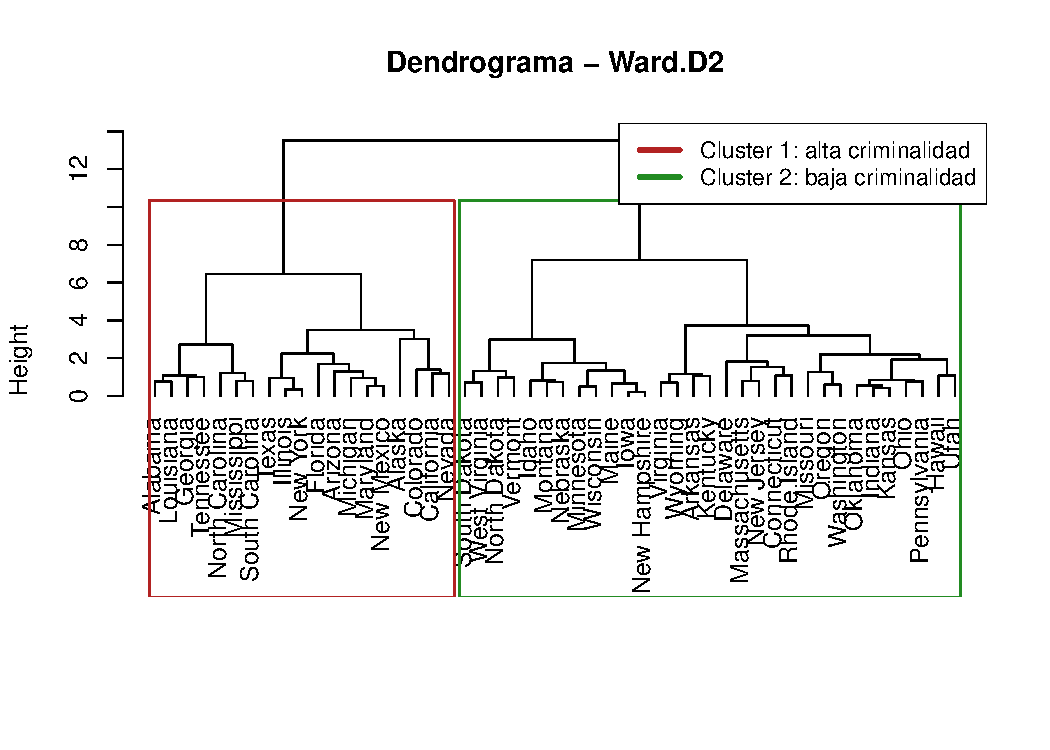
\includegraphics[keepaspectratio]{Cluster-Discriminante_files/figure-pdf/fig-clust-dend-1.pdf}}

}

\caption{\label{fig-clust-dend}Dendrograma (clustering jerárquico,
método Ward.D2 sobre variables estandarizadas)}

\end{figure}%

El dendrograma obtenido refleja la estructura jerárquica de similitud
entre los estados, basado en las tasas de criminalidad y urbanización,
utilizando el método de enlace Ward.D2 (ver
Figura~\ref{fig-clust-dend}).

El Cluster 1 reúne estados del Sur y Sureste de Estados Unidos, como
\emph{Alabama, Louisiana, Georgia, Texas} y \emph{Mississippi}, además
de grandes áreas urbanas como \emph{California, New York} e
\emph{Illinois}. Estos presentan valores positivos en todas las
variables, indicando una mayor intensidad de criminalidad y un grado de
urbanización ligeramente superior.

Por otro lado, el Cluster 2 grupa principalmente estados del Norte,
Centro-Norte y Noreste, como \emph{Montana, Dakota del Norte, Dakota del
Sur, Iowa} y \emph{Minnesota}, junto con otros de menor población y
criminalidad relativa. Este grupo se caracteriza por valores negativos
en Murder, Assault y Rape, lo que refleja una menor incidencia delictiva
y contextos más seguros.

En conjunto, los resultados muestran una división clara entre estados
con baja criminalidad y aquellos con niveles más altos, que coincide
parcialmente con un gradiente geográfico norte--sur.

\section{Análisis discriminante
(LDA)}\label{anuxe1lisis-discriminante-lda}

\section{Conclusiones (Clúster /
LDA)}\label{conclusiones-cluxfaster-lda}

El análisis de agrupamiento permitió identificar dos grupos bien
diferenciados de estados en el conjunto \emph{USArrests}, basados en
variables de criminalidad y urbanización. Un grupo esta conformado por
estados con niveles relativamente bajos de homicidios, asaltos y delitos
sexuales, junto con una urbanización ligeramente menor. Estos pueden
considerarse estados de baja criminalidad, donde los indicadores
sociales y demográficos tienden a reflejar mayor estabilidad.

En cambio, el otro grupo está compuesto por estados con valores
claramente superiores al promedio en todas las dimensiones de violencia,
sugiriendo contextos de alta criminalidad. Este grupo también presenta
una leve mayor proporción de población urbana, aunque esta diferencia no
parece ser el principal factor de separación entre los grupos.

En conjunto, ambos métodos de agrupamiento (k-means y jerárquico)
revelan un contraste consistente entre regiones de alta y baja
criminalidad, evidenciando patrones geográficos y socioeconómicos
subyacentes en los datos.




\end{document}
